\documentclass[c,18pt]{beamer}
\listfiles

\mode<presentation>
{
  \usetheme[deutsch,titlepage0]{KIT}
  \setbeamercovered{transparent}
  \setbeamertemplate{enumerate items}[ball]
}
\usepackage[utf8]{inputenc}
\date{16.10.2018}

\newlength{\Ku}
\setlength{\Ku}{1.43375pt}

\usepackage{templateSlide/exercises}
\usepackage[java]{code}

\makeatletter
\def\input@path{{uebungsfolien/}}
\graphicspath{{uebungsfolien/}}
\makeatother

%% title slide
\title[Übung 00: Einstieg in die Informatik und algorithmische]
  {Übung 00: Einstieg in die Informatik und algorithmische \\ Mathematik}
\subtitle{Albert Mink | Wintersemester 2018/2019}

\author[Albert Mink, ]{KIT}

\AuthorTitleSep{\relax}

\institute[Institut für Angewandte und Numerische Mathematik (IANM)]{Institut für Angewandte und Numerische Mathematik}

\TitleImage[width=\titleimagewd]{logos/KIT-Titel}
\logo{
\includegraphics{logos/lbrg_logo}}

%%%%%%%%%%%%%%%%%%%%%%%%%%%%%%%%%%%%%%%%%%%%%%%%%%%%%%%%%%%%%%%%%%%%%%%%
% Document
%%%%%%%%%%%%%%%%%%%%%%%%%%%%%%%%%%%%%%%%%%%%%%%%%%%%%%%%%%%%%%%%%%%%%%%%
\begin{document}
\begin{frame}
  \maketitle
\end{frame}
%%%%%%%%%%%%%%%%%%%%%%%%%%%%%%%%%%%%%%%%%%%%%%%%%%%%%%%%%%%%%%%%%%%%%%%%

\begin{frame}
  \frametitle{Arbeitsblatt 0}%
\tableofcontents[hideallsubsections]
\end{frame}

\def\kap{1}%
%\AtBeginSection{}
%%%%%%%%%%%%%%%%%%%%%%%%%%%%%%%%%%%%%%%%%%%%%%%%%%%%%%%%%%%%%%%%%%%%%%%%
\section{Einführung}
\begin{frame}
  \frametitle{\kap. Einführung}%
\tableofcontents[current]
\end{frame}


%%%%%%%%%%%%%%%%%%%%%%%%%%%%%%%%%%%%%%%%%%%%%%%%%%%%%%%%%%%%%%%%%%%%%%%%
\def\stitle{Die Übung}%
\subsection{\stitle}\label{S:Uebersicht}
\begin{frame}[fragile]%
  \frametitle{\kap.\ref{S:Uebersicht} \stitle}%

\heading{Inhalte der Übung}
\begin{itemize}
  \item Live programmieren von Rechnerdemos
  \item Besprechung der Arbeitsblätter
  \item Beantwortung von Fragen zur Vorlesung
  %\item Arbeitsblätter werden eine Woche vor der Übung hochgeladen
\end{itemize}
\hfill

\begin{description}[leftmargin=*,style=nextline]
  \item[\textcolor{black}{\textbf{Ansprechpartner}}]
  \item[Übung] Albert.Mink@kit.edu, Raum 210 Geb. 30.70,\\ Sprechstunde: nach Vereinbarung
  \item[Übung und Praktikum] Zoltan.Veszelka@kit.edu, Raum 3.014 Geb. 20.30,\\ Sprechstunde: Di, 14:00 -- 15:00
  \item[Praktikum] Ihre Tutoren im Praktikum
\end{description}
\end{frame}


%%%%%%%%%%%%%%%%%%%%%%%%%%%%%%%%%%%%%%%%%%%%%%%%%%%%%%%%%%%%%%%%%%%%%%%%
\def\stitle{Bearbeitung der Praktikumsaufgaben}%
\subsection{\stitle}\label{S:Praktikum}
\begin{frame}[fragile]%
  \frametitle{\kap.\ref{S:Praktikum} \stitle}%

\begin{itemize}
  \item Praktikumsaufgaben können zu Hause oder im Praktikum bearbeitet werden
  \item Vorbereitung \textbf{vor} dem Praktikum ist obligatorisch
  \item Tutoren \textbf{unterstützen} Sie bei Fragen und auftretenden Schwierigkeiten
  \item Sie erhalten Testate für Pflichtaufgaben die alle nachfolgenden Bedingungen erfüllen:
  \begin{itemize}
    \item Bearbeitungszeitraum ist nicht überschritten (Ausnahmen sind \textbf{nur} in begründeten Fällen möglich, z.B. Krankheit mit Attest)
    \item Programm enthält keine \emph{syntaktischen} Fehler (fehlerfrei kompilier- und ausführbar)
    \item Programm enthält keine \emph{semantischen} Fehler (es liefert die korrekten Ergebnisse)
    \item Sie können Ihr Programm \emph{live} kompilieren, ausführen \textbf{und} erklären
  \end{itemize}
\end{itemize}
\hfill

\begin{center}
 \textcolor{KITred}{Voraussetzung für die Zulassung zur Klausur:\\ Erwerb \textbf{aller} Testate}
\end{center}
\hfill

Siehe auch: Merkblatt zum Praktikum (auf ILIAS) \url{https://ilias.studium.kit.edu}
\end{frame}


%%%%%%%%%%%%%%%%%%%%%%%%%%%%%%%%%%%%%%%%%%%%%%%%%%%%%%%%%%%%%%%%%%%%%%%%
\def\stitle{Einordnung und Zusammenfassung}%
\subsection{\stitle}\label{S:Einordnung}
\begin{frame}[fragile]%
  \frametitle{\kap.\ref{S:Einordnung} \stitle}%

  \begin{tabular}{p{2cm}|p{2.0cm}|p{2.7cm}|p{3.0cm}}
  & {\centering Vorlesung} & {\centering Übung} & {\centering Praktikum}\\
  \hline
  \hline & & &  \\
  Inhalte & Vermittlung des Vorlesungs\-stoffes & Vertiefung und Wiederholung des Vorlesungsstoffes, Besprechung der Arbeitsblätter & Selbständiges Programmieren und Abgabe von Testaten (Unterstützt durch Ihre Tutoren)\\
  \hline & & & \\
  Materialien & Folien & Folien & Aufgabenblätter\\
  \hline & & & \\
  Be\-ar\-bei\-tungs\-zeit\-raum & & 1 Woche\newline (ab Dienstag) & 2 Wochen\newline  (ab Montag)\\
  %\hline & & & \\
  %Klau\-sur\-vo\-r\-aus\-set\-zung & & & Fristgerechte und erfolgreiche Abgabe \textbf{aller} Pflichtaufgaben\\
  \hline & & & \\
  Mitarbeit & wenig & mittel & viel
  \end{tabular}
  \vfill

  \textbf{Achtung:} Die ersten Tutorien finden bereits ab Montag, den 21. Oktober statt!
\end{frame}


%%%%%%%%%%%%%%%%%%%%%%%%%%%%%%%%%%%%%%%%%%%%%%%%%%%%%%%%%%%%%%%%%%%%%%%%
\def\stitle{Wichtige Termine}%
\subsection{\stitle}\label{S:Termine}
\begin{frame}[fragile]%
  \frametitle{\kap.\ref{S:Termine} \stitle}%

\begin{itemize}
  \item Vorlesung: Montags 11:30 -- 13:00
  \item Übung: Dienstags 11:30 -- 13:00
  \item Terminvergabe Praktikum: 15.Okt um 15:30 -- 17.Okt um 12:00
  \item Klausur: 23.01.20
\end{itemize}
\end{frame}

\def\kap{2}%
\AtBeginSection{}
%%%%%%%%%%%%%%%%%%%%%%%%%%%%%%%%%%%%%%%%%%%%%%%%%%%%%%%%%%%%%%%%%%%%%%%%
\section{Praktikum}
\begin{frame}
  \frametitle{\kap. Praktikum}%
\tableofcontents[currentsection]
\end{frame}
% \setcounter{section}{0}


%%%%%%%%%%%%%%%%%%%%%%%%%%%%%%%%%%%%%%%%%%%%%%%%%%%%%%%%%%%%%%%%%%%%%%%%
\def\stitle{Bearbeitung der Praktikumsaufgaben}%
\subsection{\stitle}\label{S:PraktikumSCC}
\begin{frame}[t]%
  \frametitle{\kap.\ref{S:PraktikumSCC} \stitle}%
\medskip

Praktikumsrechner des SCC
\begin{itemize}
  \item Linux Betriebssystem
  \item Software
  \begin{itemize}
    \item Eingabefenster (Shell, Terminal oder Konsole)
    \item Editor mit Syntax-Hervorhebung (z.B. Kate oder Gedit)
    \item Internet-Browser
    \item pdf-Betrachter
  \end{itemize}
  \item Kurze Einf\"uhrung: \emph{Anleitung und Informationen zum Praktikum mit den Sprachen C++ und Java} (auf ILIAS)
\end{itemize}
\end{frame}


%%%%%%%%%%%%%%%%%%%%%%%%%%%%%%%%%%%%%%%%%%%%%%%%%%%%%%%%%%%%%%%%%%%%%%%%
\def\stitle{Grundlagen der Linux Konsole}%
\subsection{\stitle}\label{S:Anleitung}
\begin{frame}[t]%
\frametitle{\kap.\ref{S:Anleitung} \stitle\ (1)}%

\heading{Generelle Bemerkungen zur Konsole}
\begin{itemize}
  \item Laufende Programme bzw. Befehlsausf\"uhrungen k\"onnen durch die Tastenkombination \textbf{Strg+c} abgebrochen werden
  \item F\"ur Autovervollst\"andigung von Dateinamen und Pfaden in der Konsole zwei Mal \textbf{Tab}
  \item F\"ur Hilfestellungen und Dokumentation \textbf{man} bzw. \textbf{-{}-help} und \textbf{google}
\end{itemize}

\end{frame}


%%%%%%%%%%%%%%%%%%%%%%%%%%%%%%%%%%%%%%%%%%%%%%%%%%%%%%%%%%%%%%%%%%%%%%%%
\begin{frame}[t]%
\frametitle{\kap.\ref{S:Anleitung} \stitle\ (2)}%
\medskip

\textbf{Die wichtigsten UNIX-Kommandos zum navigieren}
\begin{itemize}
  \setlength{\itemsep}{4pt}
  \item Aktuelles Verzeichnis ausgeben: \textbf{pwd (print working directory)}
  \item Verzeichnis wechseln: \textbf{cd (change directory)}
  \begin{itemize}
    \setlength{\itemsep}{2pt}
    \item \textbf{cd /tmp} Wechsel in das Verzeichnis /tmp (absoluter Pfad)
    \item \textbf{cd work/dat} Wechsel in das Unterverzeichnis dat von work (relativer Pfad)
    \item \textbf{cd} Wechsel in Ihr Home-Verzeichnis
    \item \textbf{cd ..} Wechsel in das \"ubergeordnete Verzeichnis
  \end{itemize}
  \item Inhalt des aktuellen Verzeichnisses auflisten: \textbf{ls (list)}
  \begin{itemize}
    \setlength{\itemsep}{2pt}
    \item \textbf{ls -{}- help} anzeigen der Dokumenation, alt. \textbf{man ls}
    \item \textbf{ls -l} zeigt Inhalt als Liste an. Verzeichnisse, Archive und ausf\"uhrbare Dateien werden eingef\"arbt
    \item \textbf{ls -lh} zeigt Inhalt zus\"atzlich als human readable an
    \item \textbf{ls -lhS} zeigt Inhalt zus\"atzlich der Gr\"o\ss e nach geordnet an
    \item $\ldots$
  \end{itemize}
\end{itemize}

\end{frame}


%%%%%%%%%%%%%%%%%%%%%%%%%%%%%%%%%%%%%%%%%%%%%%%%%%%%%%%%%%%%%%%%%%%%%%%%
\begin{frame}[t]%
\frametitle{\kap.\ref{S:Anleitung} \stitle\ (3)}%

\heading{Die wichtigsten UNIX-Kommandos zum erstellen und l\"oschen von Verzeichnissen}
\begin{itemize}
  \setlength{\itemsep}{4pt}
  \item Neues Verzeichnis anlegen: \textbf{mkdir (make directory)}
  \begin{itemize}
    \item \textbf{mkdir neu} legt das Verzeichnis neu im aktuellen Verzeichnis an
  \end{itemize}
  \item Neue Datei erstellen: \textbf{touch}
  \begin{itemize}
    \item \textbf{touch helloworld.java} erstellt die Datei helloworld.java
  \end{itemize}
  \item L\"oschen einer Datei: \textbf{rm (remove)}
  \begin{itemize}
    \setlength{\itemsep}{2pt}
    \item \textbf{rm helloworld.java} l\"oscht die Datei helloworld.java
    \item \textbf{rm -r helloworld.java} l\"oscht rekursiv, also auch gesamte Verzeichnisse
    \item \textbf{rm -f helloworld.java} erzwingt das L\"oschen
    \item \textbf{rm -v helloworld.java} aktiviert die Erkl\"arung was der Befehl bewirkt
  \end{itemize}
  \item Abrufen der Dokumentation: \textbf{man}
  \begin{itemize}
    \item \textbf{man rm} ruft die Dokumentation des Befehls \textbf{rm} auf. Mit \textbf{q (quit)} gelangt man zur\"uck.
  \end{itemize}
\end{itemize}

\end{frame}


%%%%%%%%%%%%%%%%%%%%%%%%%%%%%%%%%%%%%%%%%%%%%%%%%%%%%%%%%%%%%%%%%%%%%%%%
\begin{frame}[t]%
\frametitle{\kap.\ref{S:Anleitung} \stitle\ (4)}%

\heading{Die wichtigsten UNIX-Kommandos zum kopieren}
\begin{itemize}
  \setlength{\itemsep}{4pt}
  \item Befehl \textbf{cp (copy) [OPTION] <SOURCE> <DESTINATION>}
  \begin{itemize}
    \setlength{\itemsep}{2pt}
    \item \textbf{cp work.tex final.tex} erstellt eine Kopie von work.tex die final.tex hei\ss t
    \item \textbf{cp -r folderSource folderDest} kopiert rekursiv und damit auch Verzeichnisse
    \item Optionen: \textbf{-v, --verbose; -r, --recursive; -f, --force}
  \end{itemize}
\end{itemize}
\end{frame}


%%%%%%%%%%%%%%%%%%%%%%%%%%%%%%%%%%%%%%%%%%%%%%%%%%%%%%%%%%%%%%%%%%%%%%%%
\def\stitle{Programmentwicklung}%
\subsection{\stitle}\label{S:Progentw}
\begin{frame}[fragile]%
\frametitle{\kap.\ref{S:Progentw} \stitle}%

\heading{\"Ubersetzen des Programms}
\begin{itemize}
  \item \textbf{Wichtig:} Java Programme m\"ussen mit .java enden
  \item Java-Quelltext wird durch Aufruf des Java-Compilers in Java-Bytecode übersetzt \code{javac Dateiname.java}
  \item Zur Programm Ausf\"uhrung muss der Java-Interpreter aufgerufen werden \code{java Dateiname}
\end{itemize}

\heading{Beispiel: Kugelvolumen}
\begin{itemize}
  \item Der Java-Quelltext befindet sich in der Datei \code{KugelVolumen.java}
  \item Mit \code{javac KugelVolumen.java} wird der Quelltext in Bytecode übersetzt
  \item Der Aufruf \code{java KugelVolumen} startet das Programm in der Java Virtual Machine
  \item Auf dem Bildschirm erscheint folgende Ausgabe:
  \begin{lstlisting}[style=bash]
  Bitte Kugelradius eingeben:
  > 1
  Das Volumen betreagt v = 4.1887902047863905
  \end{lstlisting}
\end{itemize}
\end{frame}

\def\kap{3}%
\AtBeginSection{}
%%%%%%%%%%%%%%%%%%%%%%%%%%%%%%%%%%%%%%%%%%%%%%%%%%%%%%%%%%%%%%%%%%%%%%%%
\section{Installation von Java und Text Editoren}
\begin{frame}
  \frametitle{\kap. Installation von Java und Text Editoren}%
\tableofcontents[current]
\end{frame}
% \setcounter{section}{0}


%%%%%%%%%%%%%%%%%%%%%%%%%%%%%%%%%%%%%%%%%%%%%%%%%%%%%%%%%%%%%%%%%%%%%%%%
\def\stitle{Installation von Java SE}%
\subsection{\stitle}\label{S:Compiler}
\begin{frame}[t]%
  \frametitle{\kap.\ref{S:Compiler} \stitle}%

\heading{Abhängig vom Betriebssystem variiert die Installation}
\begin{description}
  \item [Linux] \"Uber den Paketmanager, hier Ubuntu 18.04, mittels \\
  \code{\$ sudo apt install openjdk-11-jdk}
  \item[Windows] Installiere Java SE (beinhaltet JDK). Download unter \textcolor{KITblue}{\url{https://www.oracle.com/technetwork/java/javase/downloads/index.html}}
  \item[Alternativ] Ab Windows 10 v.1607 "{}Anniversary Update"{} kann das \emph{Windows Subsystem for Linux} (WSL) installiert werden.
    Damit steht unter Windows das Linux Terminal zur Verfügung.
    F\"ur die Installation siehe \textcolor{KITblue}{\url{https://docs.microsoft.com/en-us/windows/wsl/install-win10}}
    \textbf{Idee:} Editiere die Quell-Dateien in Windows, und übersetzte und führe das Programm in der Linux Konsole aus.
\end{description}

\vfill
In der Übung werden die Programme mit WSL/WSL2 entwickelt.
\end{frame}


%%%%%%%%%%%%%%%%%%%%%%%%%%%%%%%%%%%%%%%%%%%%%%%%%%%%%%%%%%%%%%%%%%%%%%%%
\def\stitle{Editoren}%
\subsection{\stitle}\label{S:Editor}
\begin{frame}[t]%
  \frametitle{\kap.\ref{S:Editor} \stitle}%

Den Quelltext eines Java-Programms k\"onnen Sie mit jedem Texteditor erstellen.
Achten Sie aber darauf, dass nur der reine Text und keine Formatierungen gespeichert wird (\textbf{keine} Textverarbeitungssoftware wie MS Word, LibreOffice).
\medskip

\heading{Geeigneter Editor unter Windos}
\begin{description}
  \item[Notepad++] Open-source Texteditor f\"ur Windows mit Syntax-Highlighting.
\end{description}

\heading{Geeignete Editoren unter Linux}
\begin{description}
  \item[gedit] Dieser Editor ist auf GNOME Desktop Umgebungen vorinstalliert, somit auf den Linux Distributionen Fedora und Ubuntu.
  \item[vim] Vim ist ein konsolen-basierter Editor.
\end{description}

\vfill
Für die Programm Entwicklung mit WSL eignet sich Notepad++.
\end{frame}


%%%%%%%%%%%%%%%%%%%%%%%%%%%%%%%%%%%%%%%%%%%%%%%%%%%%%%%%%%%%%%%%%%%%%%%%
\def\stitle{Entwicklungsumgebungen}%
\subsection{\stitle}\label{S:IDE}
\begin{frame}[t]%
  \frametitle{\kap.\ref{S:IDE} \stitle}%

\heading{\textcolor{KIT-Rot}{Erfahrene} Programmierer arbeiten oft mit Entwicklungsumgebung (IDE: Integrated Development Environment).}

\begin{description}
  \item[Eclipse] Eine weitverbreitete open-source Entwicklungsumgebung die große Unterstützung aus der Industrie erhält, unter anderen von IBM, Bosch, CA Technologies, SAP, Oracle, siehe \textcolor{KITblue}{\url{www.eclipse.org}}.
  \item[NetBeans] Eine plattformunabh\"angige Entwicklungsumgebung, die im Rahmen eines von der Firma Sun Microsystems gef\"orderten Projekts entwickelt wird, siehe \textcolor{KITblue}{\url{www.netbeans.org}}.
\end{description}
\end{frame}

\def\kap{4}%
\def\stitle{Hello World}
%%%%%%%%%%%%%%%%%%%%%%%%%%%%%%%%%%%%%%%%%%%%%%%%%%%%%%%%%%%%%%%%%%%%%%%%
\section{\stitle}
\begin{frame}
  \frametitle{\kap. \stitle}%
\tableofcontents[current]
\end{frame}


%%%%%%%%%%%%%%%%%%%%%%%%%%%%%%%%%%%%%%%%%%%%%%%%%%%%%%%%%%%%%%%%%%%%%%%%
\begin{frame}[fragile]%
  \frametitle{\kap. \stitle\ - Quelltext}%

\lstinputlisting[style=JAVA,title=Diese kleine minimal Beispiel hei\ss t HelloWorld und gibt "Hello World!"{} auf der Konsole aus.]
{helloWorld/HelloWorld.java}
\end{frame}


%%%%%%%%%%%%%%%%%%%%%%%%%%%%%%%%%%%%%%%%%%%%%%%%%%%%%%%%%%%%%%%%%%%%%%%%
\begin{frame}[fragile]%
  \frametitle{\kap. \stitle\ - \"Ubersetzen und Ausf\"uhren}%

\begin{lstlisting}[title={Um das Programm HelloWorld auszuf\"uhren werden folgende Schritte auf dem Terminal durchgef\"uhrt.},style=BASH]
$ javac HelloWorld.java
$ java HelloWorld
Hello World!
\end{lstlisting}
\end{frame}

%% TODO kompilieren, mit Fehlern

\def\kap{5}%
\AtBeginSection{}
%%%%%%%%%%%%%%%%%%%%%%%%%%%%%%%%%%%%%%%%%%%%%%%%%%%%%%%%%%%%%%%%%%%%%%%%
\section{Beispiel Kugelvolumen}
\begin{frame}
  \frametitle{\kap. Beispiel Kugelvolumen}%
\tableofcontents[current]
\end{frame}


%%%%%%%%%%%%%%%%%%%%%%%%%%%%%%%%%%%%%%%%%%%%%%%%%%%%%%%%%%%%%%%%%%%%%%%%
\def\stitle{Definition Kugelvolumen}%
\subsection{\stitle}\label{S:BeispielKugelvolumen}
\begin{frame}[t]%
  \frametitle{\kap.\ref{S:BeispielKugelvolumen} \stitle}%
\medskip

Das Kugelvolumen $V$ ist der Rauminhalt einer Kugel und abh"angig vom Kugelradius $r>0$ und ist beschrieben durch
$$ V(r) := \frac{4}{3} \pi r^3. $$
\begin{itemize}
  \item Schreiben Sie ein Java-Programm, welches das Kugelvolumen einer beliebigen Kugel berechnet.
\end{itemize}
\medskip

Vorgehen:
\begin{itemize}
\item Lese Variable $r$ ein
\item W\"ahle geeigneten Datentyp f"ur Volumen $V$
\item Lade Wert von $\pi$ aus Bibliothek
\item Berechne Volumen
\item Gebe berechneten Wert auf Konsole aus
\end{itemize}
\end{frame}


%%%%%%%%%%%%%%%%%%%%%%%%%%%%%%%%%%%%%%%%%%%%%%%%%%%%%%%%%%%%%%%%%%%%%%%%
\def\stitle{Beispiel Programm}%
\subsection{\stitle}\label{S:BeispielProgramm}
\begin{frame}[t]%
  \frametitle{\kap.\ref{S:BeispielProgramm} \stitle}%
\heading{Lese Kugelradius $r$ ein}

\lstinputlisting[style=JAVAlines,frame=single,linerange={1-10, 13-14}]
{\getexercisefolder/KugelVolumen.java}
\end{frame}


%%%%%%%%%%%%%%%%%%%%%%%%%%%%%%%%%%%%%%%%%%%%%%%%%%%%%%%%%%%%%%%%%%%%%%%%
\def\stitle{Schritt f\"ur Schritt}%
\subsection{\stitle}\label{S:SchrittSchritt}
\begin{frame}[t]%
  \frametitle{\kap.\ref{S:SchrittSchritt} \stitle}%

\heading{Lade Wert $\pi$ aus Bilbliothek und berechne das Volumen}

\lstinputlisting[style=JAVAlines,frame=single,linerange={1-11, 13-14}]
{\getexercisefolder/KugelVolumen.java}

\end{frame}


%%%%%%%%%%%%%%%%%%%%%%%%%%%%%%%%%%%%%%%%%%%%%%%%%%%%%%%%%%%%%%%%%%%%%%%%
\def\stitle{Schritt f\"ur Schritt}%
\begin{frame}[t]%
  \frametitle{\kap.\ref{S:SchrittSchritt} \stitle}%

\heading{Gebe das Volumen auf Konsole aus}
\lstinputlisting[style=JAVA,linerange={1-14}]
{\getexercisefolder/KugelVolumen.java}

\end{frame}


%%%%%%%%%%%%%%%%%%%%%%%%%%%%%%%%%%%%%%%%%%%%%%%%%%%%%%%%%%%%%%%%%%%%%%%%
\def\stitle{Schritt f\"ur Schritt}%
\begin{frame}[fragile]%
  \frametitle{\kap.\ref{S:SchrittSchritt} \stitle}%
\medskip

\begin{lstlisting}[title={Um das Programm \code{KugelVolumen} auszuf\"uhren werden folgende Schritte auf dem Terminal durchgef\"uhrt.},style=BASH]
$ javac KugelVolumen.java
$ java KugelVolumen
Bitte Kugelradius eingeben: 1
Das Volumen betraegt v = 4.1887902047863905
\end{lstlisting}

\end{frame}

\def\kap{6}%
\AtBeginSection{}
%%%%%%%%%%%%%%%%%%%%%%%%%%%%%%%%%%%%%%%%%%%%%%%%%%%%%%%%%%%%%%%%%%%%%%%%
\section{Dokumentation}
\begin{frame}
  \frametitle{\kap. Dokumentation}%
\tableofcontents[current]
\end{frame}
% \setcounter{section}{0}


%%%%%%%%%%%%%%%%%%%%%%%%%%%%%%%%%%%%%%%%%%%%%%%%%%%%%%%%%%%%%%%%%%%%%%%%
\def\stitle{Java SE 8 Dokumentation}%
\subsection*{\stitle}\label{S:Java SE 8 Dokumentation}
\begin{frame}[t]%
  \frametitle{\kap.\ref{S:Java SE 8 Dokumentation} \stitle}%
\medskip

\begin{itemize}
\item Vollst\"andige Dokumentation \textcolor{KITblue}{\url{http://docs.oracle.com/javase/8/docs/api/}}
\item Umfassende Internet Tutorien \textcolor{KITblue}{\url{https://www.tutorialspoint.com/java/}} oder \textcolor{KITblue}{\url{https://www.javatpoint.com/java-tutorial}}
\end{itemize}
\medskip

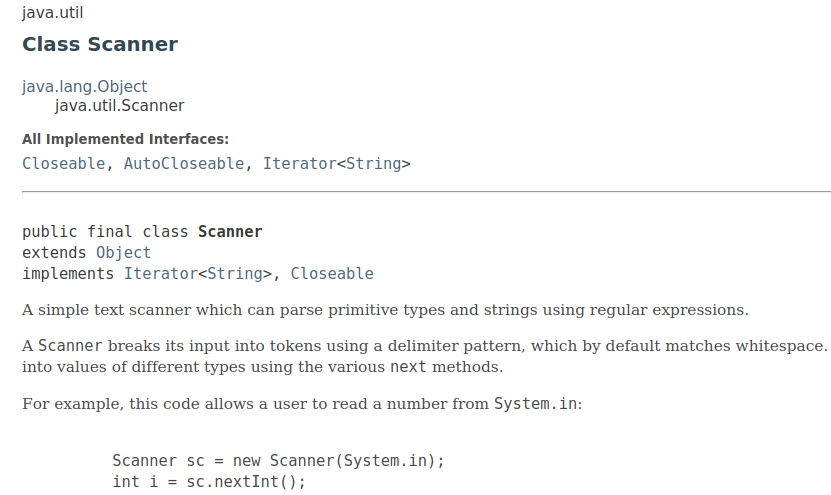
\includegraphics[width=0.8\textwidth]{\getexercisefolder/java_small.png}
\end{frame}


%%%%%%%%%%%%%%%%%%%%%%%%%%%%%%%%%%%%%%%%%%%%%%%%%%%%%%%%%%%%%%%%%%%%%%%%
\def\stitle{Online Compiler}%
\subsection*{\stitle}\label{S:Online Compiler}
\begin{frame}[t]%
  \frametitle{\kap.\ref{S:Online Compiler} \stitle}%
\medskip

Auf der Seite \textcolor{KITblue}{\url{https://www.onlinegdb.com/online_java_compiler}} k\"onnen Sie sehr bequem kleinere Programme compilieren und ausf\"uhren.
Einzige Voraussetzung ist dabei eine bestehende Internet Verbindung.
\end{frame}



%\begin{frame}
%  \frametitle{Zusammenfassung}%
%\tableofcontents[hideallsubsections]
%\end{frame}

\begin{frame}
\centering
\Huge\textcolor{KITgreen}{Fragen?}
\vspace{2cm}

{\LARGE
N\"achste \"Ubung: 23. Oktober\\
Besprechung Arbeitsblatt 1
}
\end{frame}


%%%%%%%%%%%%%%%%%%%%%%%%%%%%%%%%%%%%%%%%%%%%%%%%%%%%%%%%%%%%%%%%%%%%%%%%
\end{document}
